\documentclass[a4paper,twocolumn]{article}
\usepackage[utf8]{inputenc}
\usepackage{booktabs}
\usepackage{xcolor}
\usepackage{listings}
\usepackage{microtype}
\usepackage{tikz}
\usepackage{tikz-qtree}
\usetikzlibrary{shapes,patterns,positioning}
\usepackage{minted}
\usepackage{hyperref}

\title{Reverse Polish Notation and Stack Machines}
\author{Patrick M. Elsen <pelsen@xfbs.net>}
\date{\today}


\begin{document}
\maketitle
\tableofcontents

\section{Overview}

Reverse Polish Notation is a way to write down equations without needing to use brackets or precedence rules. This greatly simplifies parsing. For this reason, reverse polish notation has been quite popular with Casio calculators.

Take a simple mathematical equation with the four primitive operators — addition, subtraction, multiplication and division.

\begin{equation}
  \frac{(1 + 2) * (7 - 3)}{2 * 6}
\end{equation}

The rules dictate the order in which the operations should be executed, and brackets can be used to override those rules where necessary. For example, $1 + 2 * 2 - 3$ is equivalent to $1 + (2 * 2) - 3$, because multiplication has higher precedence than addition. The PEDMAS mnemonic is a good way to remember the order of precedence: \emph{parentheses, exponentiation, division, multiplication, addition, subtraction}. 

This equation could be represented in reverse polish notation as well.

\begin{equation}
1\quad2\quad+\quad7\quad3\quad-\quad*\quad2\quad6\quad*\quad/  
\end{equation}

To the uninitiated, this might seem strange, because the properties of this are not yet clear. When evaluating this, it goes strictly from left to right. Numbers are treated as data and placed on an imagined stack. Operators like $+$ (addition) consume data (numbers) from the stack, and place their results back on it. Thus, evaluating a sequence like $1\quad2\quad+$ would go like such.

\begin{table}[h!]
\begin{tabular}{@{}clp{4cm}@{}}
\toprule
Operation & Stack & Comment\\
\midrule
1 & 1 & Place 1 on stack.\\
2 & 1, 2 & Place 2 on stack.\\
$+$ & 3 & Add last two numbers on stack.\\
7 & 3, 7\\
3 & 3, 7, 3\\
- & 3, 4\\
* & 12\\
2 & 12, 2\\
5 & 12, 2, 6\\
* & 12, 12\\
/ & 1\\
\bottomrule  
\end{tabular}
\end{table}

The last result that is left on the stack is the result of the calculation, in this case 1.

Another way to think about reverse polish notation is that equations are basically tree structures, and reverse polish notation is just another way to represent the tree.

\begin{center}
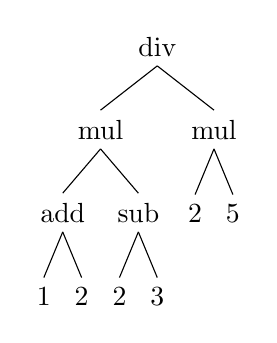
\begin{tikzpicture}
\Tree [.div [.mul [.add 1 2 ] [.sub 2 3 ] ] [.mul 2 5 ] ]
\end{tikzpicture}
\end{center}

\section{Evaluating}

With the knowledge of how reverse polish notation looks like, it's fairly trivial to parse and interpret it. Given a function that splits a string into individual tokens, and some classes to represent the operations, parsing RPN is as simple as a few if statements.

\begin{minted}{cpp}
if(tok == "+") {
    return new Add();
} else if(tok == "*") {
    return new Mul();
} else if(tok == "-") {
    return new Sub();
} else if(tok == "/") {
    return new Div();
}

return new Num(std::stod(tok));
\end{minted}

To represent the stack, the C++ \verb|std::deque<double>| is a good candidate, because it acts like a stack (meaning that it has efficient pop and push operations) but it also allows index-based access to elements, which is useful for displaying the stack.

With this in mind, the execute functions for the number token can look somewhat like this, simply pushing the data onto the stack.

\begin{minted}{cpp}
void Num::execute(std::deque<double> &s) {                                                                                                                                                           
    s.push_back(number);                                                                                                                                                                                
}  
\end{minted}

Similarly, the other operations can be implemented, by popping values off the stack and pushing the result back onto it.

\begin{minted}{cpp}
void Add::execute(std::deque<double> &s) {
    double rhs = s.back();
    s.pop_back();
    double lhs = s.back();
    s.pop_back();
    s.push_back(lhs + rhs);
}  
\end{minted}

There is example code in the \verb|calc| folder in this repository with working code that acts as a little reverse polish notation parser. Compiling that and playing with it might help.

After every sequence of tokens, it prints out the entire stack, making examining the state very easy.

\begin{verbatim}
$ cd calc/
$ mkdir build && cd build/
$ cmake .. && make
$ ./calc-cli
> 1 2 +
3
> 3 4 +
3 7
> +
10
> 5 6 +
10 11
> 7 8 +
10 11 15
> +
10 26
> +
36
\end{verbatim}

This particular interpreter only supports the four basic math operators, but it is very simple to extend the code to make it support more.

In fact, there are existing reverse polish notation interpreters and compilers that support a lot more. There's even one on your printer right now -- we'll get to that one in a bit.

\subsection{DC}

DC might just be the oldest and yet most universal reverse polish notation interpreter. Its name is an acronym for \emph{desktop calculator}, and that is exactly what it does.

You can pop open the manual page for \verb|dc| to get a bit of information about it.

\begin{verbatim}
$ man dc
\end{verbatim}

It looks really quite cryptic, especially because it is character-based. It can do simple addition like we did before. One difference is that it does not implicitly print the stack -- but the \verb|p| command exists to print the stack.

\begin{verbatim}
$ dc -e "1 2 3 + + p"
6
\end{verbatim}

Looking at the manual page, it becomes evident that it can do a lot more than that. 


\section{Generating}

Reverse polish notation is


Reverse polish notation in dc



\end{document}
